\section{Trasformata di Burrows--Wheeler posizionale}
\label{secpbwt}
Presentata nel 2014 da Richard Durbin \cite{pbwt}, la \textbf{Positional
  Burrows--Wheeler Transform} ($\PBWT$), traducibile con
\textit{trasformata di Burrows--Wheeler posizionale}, è una struttura efficiente
per la memorizzazione e l'interrogazione di pannelli di aplotipi.\\
La costruzione di tali pannelli avviene tramite il riconoscimento delle
variazioni di un singolo nucleotide tra le sequenze genomiche di diversi
individui, ovvero dei cosiddetti Single-Nucleotide Polymorphism
(SNP). Ogni variazione, identificata per un certo nucleotide in una
posizione specifica, viene 
detto allele. La combinazione di tutte le varianti alleliche,
ereditate, a meno di mutazioni, da ogni genitore, forma l'\textbf{aplotipo} di
un certo individuo. Come visibile in figura \ref{fig:haplo} \cite{haplo}, la 
costruzione parte dai
vari sequenziamenti (nell'immagine relativi a diversi cromosomi ma il
procedimento è uguale partendo da diversi individui) da cui si identificano le
varianti alleliche. Da queste ultime si costruiscono gli aplotipi, da cui si
estraggono i cosiddetti tag SNP, ovvero le possibili alternative per
una certa variante allelica. Questi ultimi, normalmente rappresentati per
l'uomo da due caratteri vista la sua natura diploide, formano,
l'alfabeto del pannello. 
L’informazione combinata di tutti gli aplotipi in un individuo è detta,
invece, \textbf{genotipo}.
\begin{figure}
  \centering
  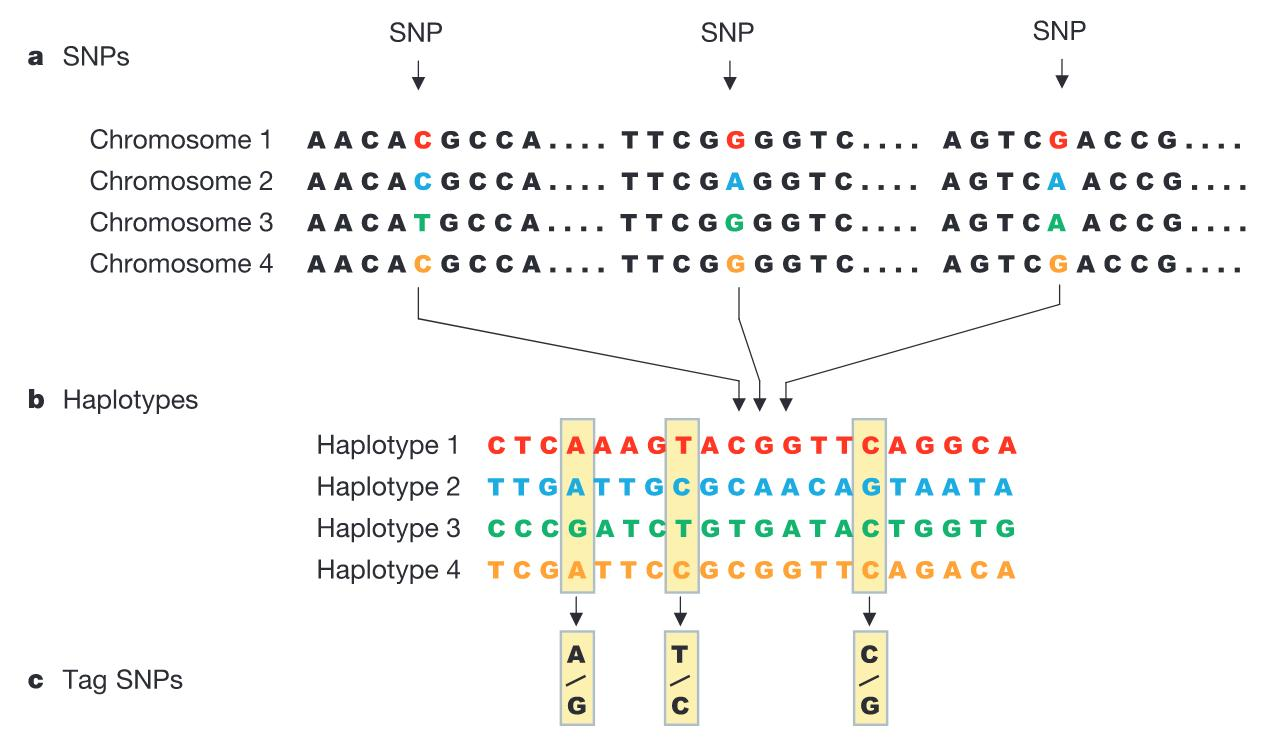
\includegraphics[scale = 0.3]{img/haplo.jpg}
  \caption{Schema di ottenimento del pannello di aplotipi.}
  \label{fig:haplo}
\end{figure}
Formalmente, si considera un pannello $X$ di $M$ aplotipi $x_i$, con
$i=0,\ldots, M-1$, su $N$ siti, indicizzati tramite $k=0,\ldots, N-1$, tale per
cui tutti i siti sono considerati biallelici. 
Da un punto di vista computazionale, quest'ultima
assunzione comporta che il pannello $X$ è costruito sull'alfabeto ordinato
$\Sigma =\{0,1\}$, con $0\prec 1$, avendo la sostituzione dei tag SNPs,
per un certo sito, con tale alfabeto. Ne segue che:
\begin{equation}
  \label{eq:pbwtdip}
  x_i[k]=\{0,1\}
\end{equation}
Prima di proseguire con la trattazione è bene fornire la descrizione di alcuni
formalismi utilizzati:
\begin{itemize}
  \item si denota, per una qualsiasi riga $x_i$, con $x_i[k_1,k_2)$ la
  sottostringa di $x_i$ che inizia alla colonna $k_1$ e termina alla
  colonna $k_2-1$
  \item date due righe $x_i$ e $x_j$, si definisce un match tra le due
  righe, iniziante
  alla colonna $k_1$ e terminante alla colonna $k_2-1$, sse:
  \begin{equation}
    \label{eq:pbwtmatch}
    x_i[k_1,k_2)=x_j[k_1,k_2)
  \end{equation}
  \item un match tra due righe $x_i$ e $x_j$, come definito al punto precedente,
  è definito localmente massimale sse non si ha alcuna estensione a
  destra o sinistra che comporti un ulteriore match:
  \begin{equation}
    \label{eq:pbwtmem}
    (k_1=0\lor x_i[k_1-1]\neq x_j[k_1-1])\land (k_2=N\lor x_i[k_2]\neq x_j[k_2])
  \end{equation}
  \item comparando una sequenza $z$ ad un pannello di aplotipi $X$, si definisce
  set-maximal exact match ($\SMEM$) di $z$ contro $x_i\in X$ un match
  localmente massimale, iniziante 
  alla colonna $k_1$ e terminante alla colonna $k_2-1$,
  sse non si ha alcun altro match localmente
  massimale di $z$ con un 
  altro $x_j$ che include ed estende l'intervallo $[k_1,k_2)$. La sequenza $z$
  può avere uno $\SMEM$, tra $k_1$ e $k_2-1$, con più di un aplotipo del
  pannello. Per praticità, si è introdotta la definizione di $\SMEM$ usando un
  aplotipo esterno. Tale definizione può essere riferita anche a due righe
  interne al pannello $X$
\end{itemize}
Si noti che il match tra due sequenze nella $\PBWT$ è tale sse iniziano
entrambi nella stessa colonna e terminano nella stessa colonna. Questo vincolo,
da cui deriva il termine ``posizionale'' e che, di fatto, impedisce l'uso degli
algoritmi tradizionali visti con la $\BWT$, è dato dal fatto che una
colonna rappresenta un preciso sito di una variante genica. \\
La costruzione di questa struttura dati si basa, ad ogni colonna $k$, sul
riordinamento lessicografico delle sequenze di aplotipi basato sull'ordinamento
inverso dei prefissi terminanti in colonna $k-1$. I valori presenti in colonna
$k$, dopo il riordinamento, altro non sono che i valori che andranno a popolare
la cosiddetta matrice $\PBWT$, che rappresenta la vera e propria
trasformata. Si noti che avere le sequenze 
ordinate in base ai prefissi invertiti alla $k$-esima colonna permette di
identificare i match con maggior facilità in quanto, ad ogni colonna, aplotipi
con suffisso comune (o prefisso comune in ordine inverso) saranno in posizioni
consecutive all'interno della trasformata.\\
La computazione di tutti i riordinamenti non presenta difficoltà dal punto di
vista computazionale in quanto, conoscendo l'ordinamento in colonna $k$, si può
derivare facilmente l'ordinamento in colonna $k+1$, studiando solo i valori
riordinati alla colonna precedente. Si ha infatti un ordinamento stabile ad ogni
colonna. 
\begin{definizione}
  Dato un aplotipo $i$, appartenente al pannello $X$, e un indice di colonna
  $k$, si definisce il \textbf{prefix array} $a_k$ come una permutazione degli
  indici $\{0,\ldots, M-1\}$ tale che $a_k[i]=j$ sse $x_j$ è l'$i$-esimo
  aplotipo di 
  $X$ nell'ordinamento inverso dei prefissi ottenuto alla colonna $k$. Quindi,
  $a_k[i]=m$, con $m<M$, altro non è che l'indice della sequenza $x_m$ del
  pannello $X$ da cui deriva il prefisso $i$-esimo nell'ordine inverso
  in colonna $k$.
\end{definizione}
Data questa definizione ne segue che la matrice $\PBWT$ si ottiene
direttamente andando a vedere, per ogni colonna, gli indici del prefix
  array e prendendo i valori del pannello $X$ secondo l'ordine espresso da
esso.\\ 
Per comodità di rappresentazione definiamo formalmente i valori della
 matrice $\PBWT$ con il seguente formalismo:
\begin{equation}
  \label{eq:pbwty}
  y_i^k[j]=x_{a_k[i]}[j]
\end{equation}
avendo quindi che $y_i^k$ denota la sequenza $i$-esima secondo l'ordinamento
ottenuto per la colonna $k$. Si può quindi accedere al valore $j$-esimo, ovvero
il valore in colonna $j$, di tale
sequenza. Si può meglio spiegare perché risulti 
semplice computare i vari prefix array. L'ordinamento degli elementi per
$a_{k+1}$ si ottiene a partire 
dall'ordinamento in $a_k$. Si considerano, infatti, i valori $y_i^k[k]$ e la
precedenza del valore 0 sul valore 1 per riordinare in modo stabile tali
valori.\\ 
\dc{Un po' confusionario}
Come anticipato, prefissi simili saranno consecutivi nei riordinamenti fino alla
colonna $k$-esima. Quindi, risulta utile tenere traccia della posizione iniziale
dei match tra prefissi vicini. 
\begin{definizione}
  Si definisce \textbf{divergence array} l'array $d_k$, tale che $d_k[i]$ è
  l'indice colonna iniziale del match massimale a sinistra terminante in $k$ tra
  l'$i$-esimo aplotipo e il suo precedente nell'ordinamento ottenuto alla
  colonna $k$-esima. Formalmente, dato $i>0$, si definisce 
  $d_k[i]$ come il più piccolo $j$ tale che:
  \begin{equation}
    \label{eq:pbwtdiv}
    y_i^k[j,k)=y_{i-1}^k[j,k)
  \end{equation}
  Ne segue che
  \begin{equation}
    \label{eq:pbwtdiv2}
    y_i^k[k-1]\neq y_{i-1}^k[k-1] \implies d_k[i]=k
  \end{equation}
  Per definizione, non avendo una riga precedente con cui effettuare il
  confronto: 
  \begin{equation}
    \label{eq:pbwtdiv3}
   d_k[0]=k
  \end{equation}
\end{definizione}
Si può quindi dimostrare che l'inizio di qualsiasi match massimale, terminante
in colonna $k$, tra qualsiasi $y_i^k$ e $y_j^k$, con $i<j$, è calcolabile
facilmente avendo che è dato da:
\begin{equation}
  \label{eq:pbwtint}
  \max_{i<m\leq j}d_k[m]
\end{equation}
Si noti che al posto del divergence array si può usare anche una
variante posizionale del Longest Common Prefix array.
\begin{definizione}
  Si definisce Reverse Longest Common Prefix ($\,\RLCP$) l'array $l_k$
  che, anziché 
  memorizzare l'indice d'inizio del match massimale a sinistra da due aplotipi
  consecutivi nell'ordinamento ottenuto alla colonna $k$-esima, tiene traccia
  della lunghezza di tale match. Formalmente si ha, quindi, che:
  \begin{equation}
    \label{eq:pbwtlcp}
    l_k[i]=k-d_k[i]
  \end{equation}
\end{definizione}
\noindent
Fatte queste premesse possiamo quindi fornire una definizione formale di
$\PBWT$.
\begin{definizione}
  Dato un pannello di $M$ aplotipi con $N$
  siti $X=\{x_1,x_2,\ldots,x_M\}$, si definisce $\PBWT$ di $X$ come una
  collezione di $N+1$ coppie di array $(a_k,d_k)$, con $0\leq k\leq N$.
\end{definizione}
La procedura per la costruzione di $a_{k+1}$ e $d_{k+1}$ a partire da $a_k$ e
$d_k$ è disponibile all'algoritmo \ref{algo:durbin1}. Si può quindi notare come
il costo della costruzione dei due insiemi di array sia:
\begin{equation}
  \label{eq:pbwtadtime}
  \mathcal{O}(NM)
\end{equation}
\dc{Serve altro? Serve spiegare i dettagli dell'algoritmo?}
\begin{algorithm}
  \small
  \begin{algorithmic}[1]
    \Function{BuildPrefixAndDivergenceArrays}{$k$, $M$, $a_k$, $d_k$}
    \State $u\gets 0$, $v\gets 0$
    \State $p\gets k+1$, $q\gets k+1$
    \State $a\gets []$, $b\gets []$, $d\gets []$, $e\gets []$
    \For {\textit{every} $i\in[0,M-1]$}
    \If {$d_k[i]>p$}
    \State $p\gets d_k[i]$
    \EndIf
    \If {$d_k[i]>q$}
    \State $q\gets d_k[i]$
    \EndIf
    \If {$y_i^k[k]=0$}
    \State $a[u]\gets a_k[i]$, $d[u]\gets p$
    \State $u\gets u+1$, $p\gets 0$
    \Else
    \State $b[v]\gets a_k[i]$, $e[v]\gets q$
    \State $v\gets v+1$, $q\gets 0$
    \EndIf
    \EndFor
    \State $a_{k+1}\gets concatenate(a,b)$
    \State $d_{k+1}\gets concatenate(d,e)$ 
    \EndFunction
  \end{algorithmic}
  \caption{Algoritmo di Durbin per la costruzione di $a_{k+1}$ e $d_{k+1}$ a
  partire da $a_{k}$ e $d_{k}$.}
  \label{algo:durbin1}
\end{algorithm}
Ai fini della trattazione dell'algoritmo di match con un'aplotipo esterno
ricordiamo un'ulteriore definizione.
\begin{definizione}
  Si definisce $\alpha_k$ come l'inverso della permutazione data dal
    prefix array $a_k$, avendo che:
  \[\alpha_k[i]=j \iff a_k[j]=i\]
\end{definizione}
Grazie a queste prime definizioni è possibile notare alcune prime forti
correlazioni, fattore chiave nello sviluppo di questa tesi, che sussistono tra
$\BWT$ e $\PBWT$ (e le rispettive varianti run-length
  encoded. Nella seguente tabella si ricordano queste prime correlazioni:
\begin{table}[H]
  \centering
  \begin{tabular}{c|c}
    $\BWT$ & $\PBWT$\\
    \hline
    $\SA_T$ & $a_k$\\
    $\ISA_T$ & $\alpha_k$\\
    $\LCP_T$ & $d_k$ o $l_k$\\            
  \end{tabular}
\end{table}
\begin{esempio}
  \label{es:pbwt1}
  Si assuma il seguente pannello $X$ e di voler calcolare $y^6$:
  \begin{table}[H]
    \centering
    \small
    \begin{tabular}{c|ccccccccccccccc}
      X & 00 & 01 & 02 & 03 & 04 & 05 & 06 & 07 & 08 & 09 & 10 & 11 & 12 & 13
      & 14 \\
      \hline
      00 & 1 & 0 & 0 & 1 & 0 & 0 & 0 & 0 & 0 & 0 & 0 & 1 & 1 & 0 & 1 \\
      01 & 1 & 0 & 0 & 1 & 1 & 0 & 0 & 1 & 0 & 0 & 0 & 0 & 0 & 1 & 1 \\
      02 & 1 & 0 & 0 & 1 & 1 & 0 & 0 & 1 & 0 & 0 & 0 & 1 & 0 & 0 & 1 \\
      03 & 1 & 0 & 0 & 1 & 1 & 0 & 0 & 1 & 0 & 0 & 0 & 1 & 0 & 0 & 1 \\
      04 & 0 & 1 & 0 & 1 & 0 & 1 & 0 & 0 & 0 & 0 & 0 & 1 & 0 & 0 & 1 \\
      05 & 0 & 1 & 0 & 1 & 0 & 1 & 0 & 0 & 0 & 0 & 0 & 1 & 0 & 0 & 1 \\
      06 & 0 & 1 & 0 & 1 & 0 & 1 & 0 & 0 & 0 & 0 & 0 & 1 & 0 & 0 & 1 \\
      07 & 0 & 1 & 0 & 1 & 0 & 1 & 0 & 0 & 0 & 0 & 0 & 0 & 1 & 0 & 1 \\
      08 & 0 & 1 & 0 & 0 & 1 & 0 & 0 & 0 & 0 & 1 & 1 & 1 & 0 & 0 & 1 \\
      09 & 0 & 1 & 0 & 1 & 0 & 0 & 0 & 0 & 1 & 0 & 0 & 0 & 0 & 1 & 1 \\
      10 & 0 & 1 & 0 & 1 & 0 & 0 & 0 & 0 & 1 & 0 & 0 & 0 & 0 & 1 & 1 \\
      11 & 0 & 1 & 0 & 0 & 1 & 0 & 0 & 0 & 0 & 0 & 1 & 1 & 0 & 0 & 0 \\
      12 & 0 & 1 & 0 & 0 & 1 & 0 & 0 & 0 & 1 & 0 & 1 & 1 & 0 & 0 & 1 \\
      13 & 0 & 1 & 0 & 0 & 1 & 0 & 0 & 0 & 1 & 0 & 1 & 1 & 0 & 0 & 1 \\
      14 & 0 & 1 & 0 & 0 & 0 & 0 & 0 & 0 & 1 & 0 & 0 & 0 & 1 & 0 & 1 \\
      15 & 0 & 1 & 0 & 0 & 0 & 0 & 0 & 0 & 1 & 0 & 0 & 0 & 1 & 0 & 1 \\
      16 & 0 & 1 & 0 & 1 & 0 & 0 & 0 & 0 & 0 & 0 & 0 & 1 & 1 & 0 & 1 \\
      17 & 1 & 1 & 0 & 0 & 0 & 1 & 0 & 0 & 0 & 0 & 0 & 1 & 1 & 0 & 1 \\
      18 & 0 & 1 & 1 & 0 & 1 & 0 & 0 & 0 & 0 & 0 & 0 & 1 & 0 & 0 & 1 \\
      19 & 0 & 1 & 1 & 0 & 1 & 0 & 1 & 0 & 0 & 0 & 0 & 0 & 1 & 0 & 1 
    \end{tabular}
  \end{table}
  Si inizia riordinando il pannello con l'ordine inverso alla
  quinta colonna, avendo che $y^6$ altro non è che la sesta colonna del pannello
  così riordinato. Ne segue che $a_6$ è la colonna degli indici, che è stata
  ottenuta con la permutazione data dall'ordinamento, e $d_6$ la
  colonna iniziale in cui terminano i match tra righe consecutive nel
  rioridnamento le sottolineature (evidenziati nell'immagine seguente dalle
  sottolineature):   
  \begin{figure}[H]
    \centering
    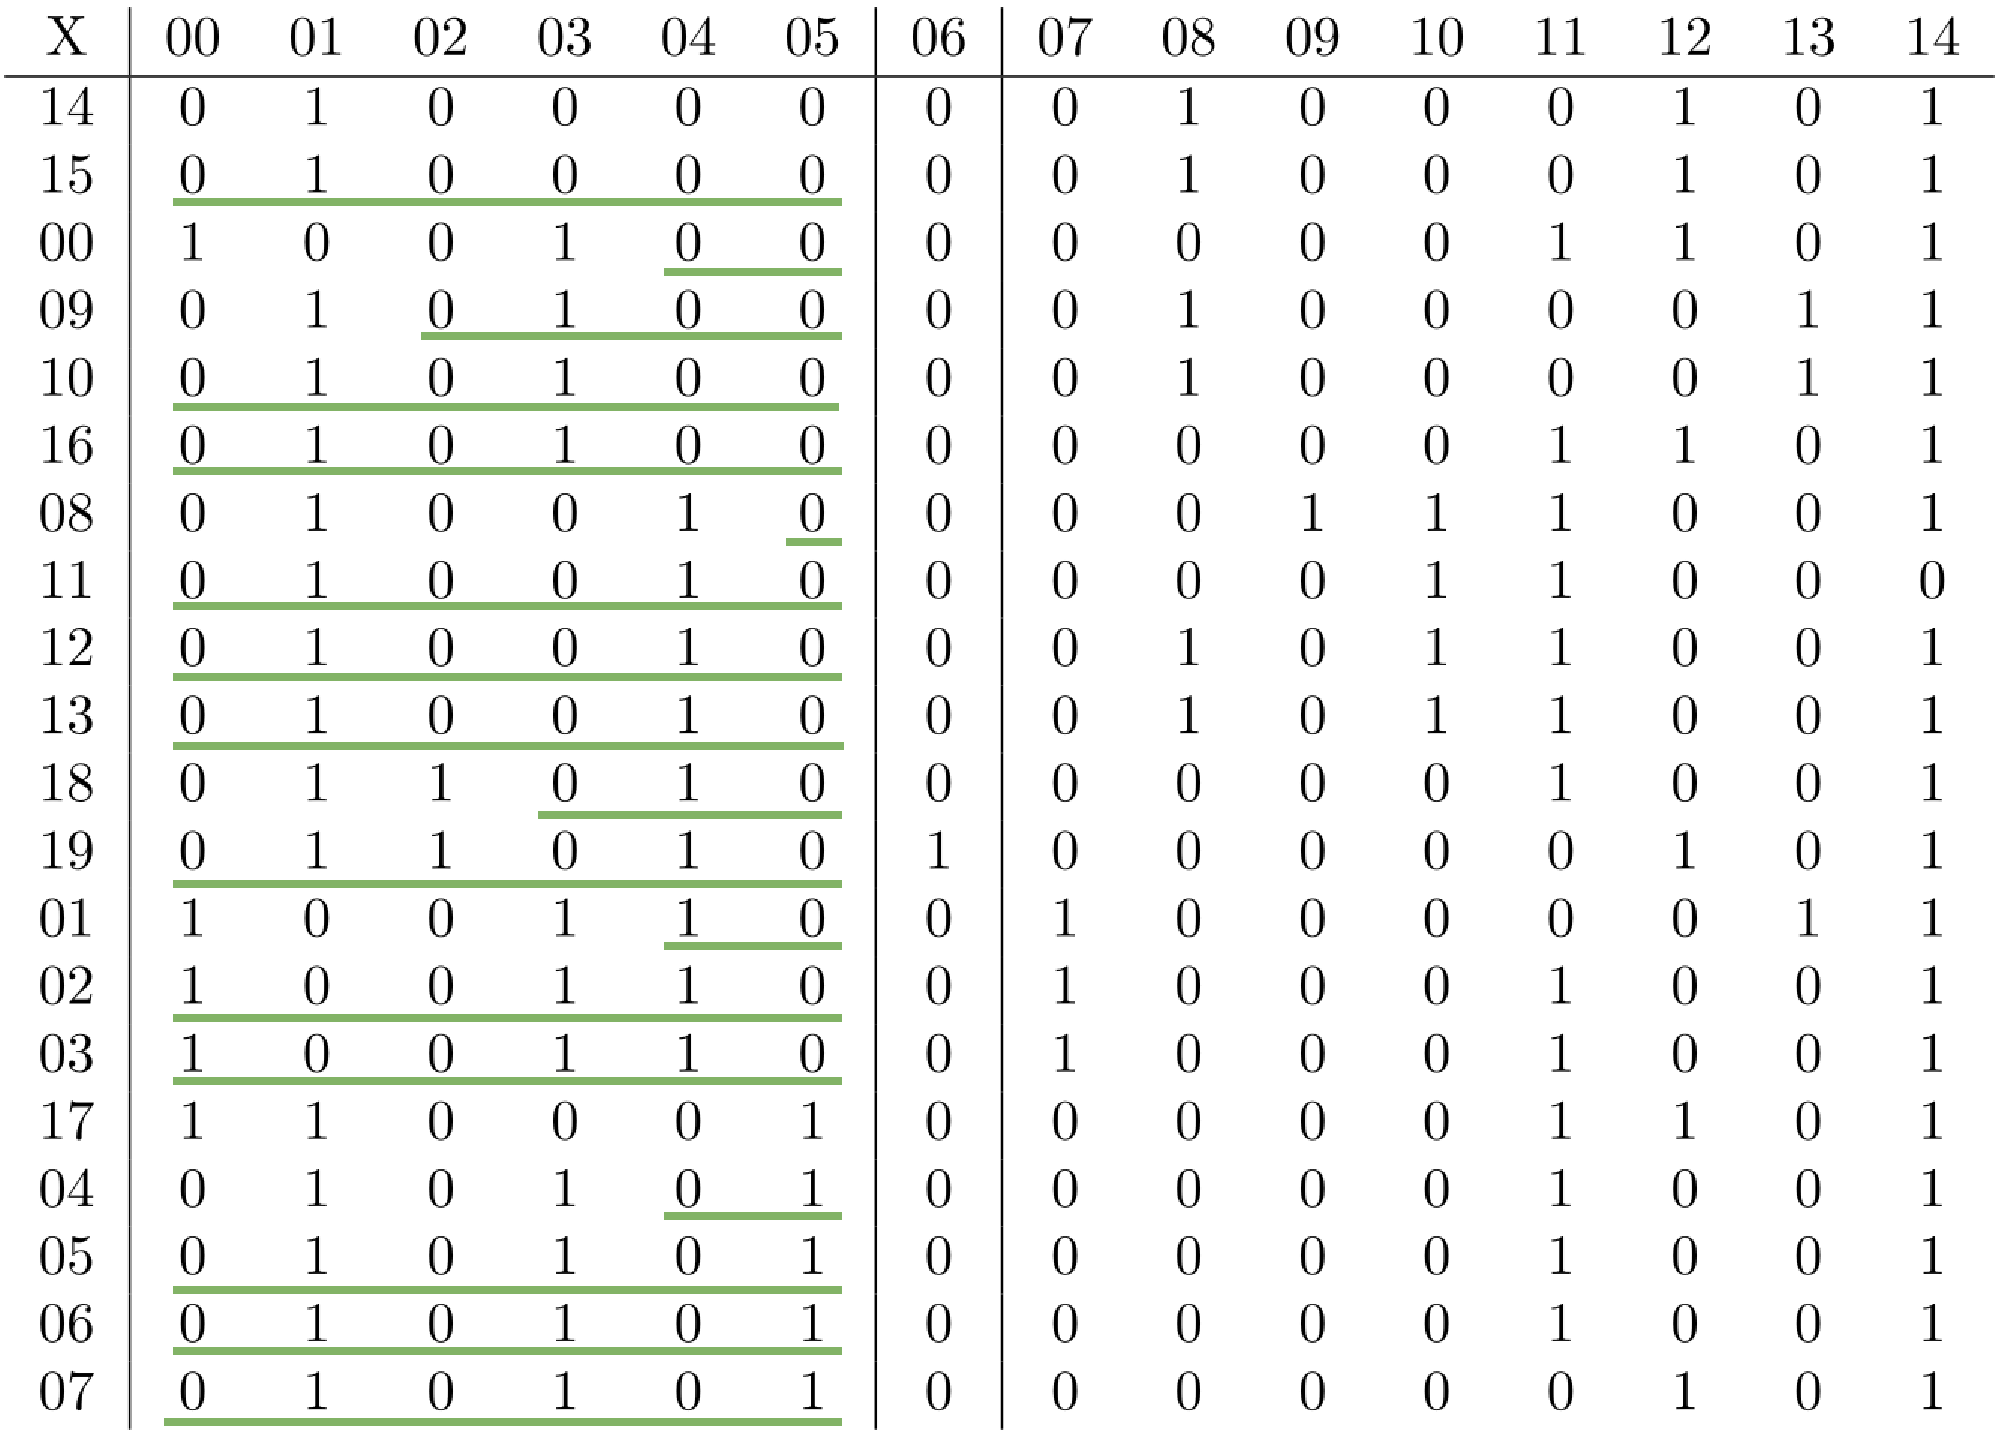
\includegraphics[scale = 0.325]{img/matrix1.pdf}
  \end{figure}
  \noindent
  Avendo, nel complesso:
  \[a_6=[14,15,0,9,10,16,8,11,12,13,18,19,1,2,3,17,4,5,6,7]\]
  \[\alpha_6=[2,12,13,14,16,17,18,19,6,3,4,7,8,9,0,1,5,15,10,11]\]
  \[d_6=[6,0,4,2,0,0,5,0,0,0,3,0,4,0,0,6,4,0,0,0]\]
  \[l_6=[0,6,2,4,6,6,1,6,6,6,3,6,2,6,6,0,2,6,6,6]\]
  Con il calcolo di tutti gli $a_k$ si otterrebbe la seguente matrice $\PBWT$:
  \begin{table}[H]
  \centering
  \scriptsize
  \begin{tabular}{c|ccccccccccccccc}
    X & 00 & 01 & 02 & 03 & 04 & 05 & 06 & 07 & 08 & 09 & 10 & 11 & 12 & 13
    & 14 \\
    \hline
    00 & 1 & 1 & 0 & 1 & 1 & 0 & 0 & 0 & 1 & 0 & 0 & 1 & 1 & 1 & 1 \\
    01 & 1 & 1 & 0 & 1 & 1 & 0 & 0 & 0 & 1 & 0 & 0 & 1 & 1 & 1 & 1 \\
    02 & 1 & 1 & 0 & 1 & 1 & 1 & 0 & 0 & 0 & 1 & 1 & 1 & 0 & 1 & 1 \\
    03 & 1 & 1 & 0 & 1 & 1 & 0 & 0 & 0 & 1 & 0 & 0 & 1 & 1 & 0 & 1 \\
    04 & 0 & 1 & 0 & 1 & 0 & 1 & 0 & 0 & 1 & 0 & 0 & 1 & 1 & 0 & 1 \\
    05 & 0 & 1 & 0 & 1 & 0 & 1 & 0 & 0 & 0 & 0 & 0 & 1 & 0 & 0 & 1 \\
    06 & 0 & 1 & 0 & 1 & 0 & 1 & 0 & 0 & 0 & 0 & 0 & 1 & 0 & 0 & 0 \\
    07 & 0 & 1 & 0 & 1 & 1 & 1 & 0 & 0 & 0 & 0 & 0 & 0 & 1 & 0 & 1 \\
    08 & 0 & 1 & 0 & 0 & 1 & 0 & 0 & 0 & 1 & 0 & 0 & 0 & 1 & 0 & 1 \\
    09 & 0 & 1 & 0 & 1 & 0 & 0 & 0 & 0 & 1 & 0 & 0 & 0 & 0 & 0 & 1 \\
    10 & 0 & 1 & 0 & 1 & 1 & 0 & 0 & 0 & 0 & 0 & 0 & 1 & 1 & 0 & 1 \\
    11 & 0 & 1 & 0 & 0 & 1 & 0 & 1 & 1 & 0 & 0 & 0 & 1 & 0 & 0 & 1 \\
    12 & 0 & 1 & 0 & 0 & 1 & 0 & 0 & 1 & 0 & 0 & 0 & 0 & 0 & 0 & 1 \\
    13 & 0 & 1 & 0 & 0 & 0 & 0 & 0 & 1 & 0 & 0 & 0 & 0 & 0 & 0 & 1 \\
    14 & 0 & 1 & 0 & 0 & 0 & 0 & 0 & 0 & 0 & 0 & 0 & 0 & 0 & 0 & 1 \\
    15 & 0 & 0 & 0 & 0 & 0 & 0 & 0 & 0 & 0 & 0 & 0 & 0 & 0 & 0 & 1 \\
    16 & 0 & 0 & 0 & 1 & 0 & 0 & 0 & 0 & 0 & 0 & 0 & 1 & 0 & 0 & 1 \\
    17 & 1 & 0 & 1 & 0 & 0 & 0 & 0 & 0 & 0 & 0 & 1 & 1 & 0 & 0 & 1 \\
    18 & 0 & 0 & 1 & 0 & 0 & 0 & 0 & 0 & 0 & 0 & 1 & 1 & 0 & 0 & 1 \\ 
    19 & 0 & 1 & 0 & 0 & 0 & 0 & 0 & 0 & 0 & 0 & 1 & 1 & 0 & 0 & 1
  \end{tabular}
\end{table}
\end{esempio}
\subsection{Set-maximal match con aplotipo esterno}
Durbin, nel suo articolo, propone diversi algoritmi per l'uso effettivo della
sua trasformata. Ad esempio, viene proposto un algoritmo per il calcolo
di match interni ad $X$ più lunghi di una lunghezza minima $L$ e uno per la
ricerca di tutti gli $\SMEM$ interni ad $X$ in tempo lineare.\\
Di interesse per questa tesi è però il cosiddetto \textbf{algoritmo 5}, che
si propone di trovare tutti gli $\SMEM$  tra il panello $X$ e un
aplotipo esterno $z$, assumendo $|z|=N$. Quest'ultimo vincolo è dovuto al fatto
che una colonna $k$ del
pannello e una posizione $k$ della query rappresentano il medesimo sito.\\ 
L'idea dietro l'algoritmo è quella di usare tre indici: $e_k$, $f_k$ e
$g_k$. Nel dettaglio $e_k$ tiene traccia dell'inizio del più lungo match,
terminante in colonna $k$, tra $z$ e un qualche $y_i^k$. L'intervallo
$[f_k,g_k)\subseteq[0,\ldots,M)$ invece identifica il sotto-intervallo di
$a_k$ contenente gli indici degli aplotipi appartenetenti a tale match. Si noti
come si riprenda quindi l'idea, vista con la backward search per la
$\BWT$, di studiare un intervallo $[f_k,g_k)$ su $\SA_T$ per identificare i
match tra un pattern e un testo. In questo caso si ha però a che fare con una
forward search.
\begin{definizione}
  Dato un pannello $X$, con $M$ aplotipi/righe e $N$ siti/colonne, e un aplotipo
  query $z$, tale che $|z|=N$, si definisce uno $\SMEM$ iniziante in colonna
  $e_k$ e terminante il colonna 
  $k$, tra 
  la query $z$ e tutte le righe del pannello indicizzate dai valori compresi
  nell'intervallo $[f_k,g_k)$ in $a_k$ sse:
  \begin{equation}
    \label{eq:pbwtsmem}
    z[e_k,k)=y_i^k[e_k,k)\land z[e_k-1]\neq y_i^k[e_k-1], \forall\, i\mbox{
      t.c. }f_k\leq i < g_k
  \end{equation}
  Si noti che $g_k=M$ sse $y_{M-1}^k$ appartiene alle righe per le quali si ha
  tale $\SMEM$.
\end{definizione}
Bisogna capire come aggiornare $e_k$, $f_k$ e $g_k$ passando dalla
colonna $k$ alla colonna $k+1$. Si procede esattamente come visto per la
backward search nella $\BWT$, selezionando, per calcolare $[f_{k+1},g_{k+1})$, il
sottointervallo di $[f_k,g_k)$ in cui si hanno aplotipi che possono essere estesi
a destra con il simbolo $z[k+1]$. L'idea è quella per cui, avendo
$f_{k+1}<g_{k+1}$ allora sicuramente ho ancora delle righe che presentano un
match che parte da $e_{k+1}=e_{k}$ e termina in $k$ che può essere esteso in
$k+1$. In caso contrario, avendo $f_{k+1}=g_{k+1}$, non si hanno match
estendibili e quindi si può concludere che quelli terminanti in colonna $k$
erano $\SMEM$. In questo secondo caso bisogna poi aggiornare $e_{k+1}$,
ottenedo i relativi valori $f_{k+1}$ e $g_{k+1}$, al fine di trovare la nuova
colonna da cui parte lo $\SMEM$ successivo e le righe del pannello per le quali
si ha tale $\SMEM$. \\
Bisogna, quindi, capire come funzioni la
variante del backward-step introdotta per la $\BWT$. Nella $\PBWT$ si può
parlare di forward-step. Tale funzione,
guidata dal carattere corrente dell'aplotipo query, permette di ottenere
$f_{k+1}$ e $g_{k+1}$ a partire da $f_k$ e $g_k$.\\ 
Per effettuare il mapping abbiamo bisogno di tre componenti, che,
intuitivamente, svolgono la medesima funzione di $\C$ e $\Occ$ per la
$\BWT$: 
\begin{enumerate}
  \item l'array $c$ tale per cui $c[k]=j$ sse la colonna $k$ contiene $j$
  occorrenze di 0
  \item l'array $u_k$ tale per cui, alla colonna $k$-esima, $u_k[i]=j$ sse $j$ è
  il numero di occorrenze di 0 prima dell'indice $i$ nella $y^k[k]$ 
  \item l'array $v_k$ tale per cui, alla colonna $k$-esima, $v_k[i]=j$ sse $j$ è
  il numero di occorrenze di 1 prima dell'indice $i$ in $y^k[k]$ 
\end{enumerate}
Tali valori possono essere computati e memorizzati in fase di costruzione della
$\PBWT$, come visibile direttamente nell'algoritmo \ref{algo:durbin1} per
quanto riguarda $u$ e $v$. Per quanto riguarda $c$
si ha che potrebbe essere banalmente calcolato anch'esso in fase di costruzione
della $\PBWT$, tenendo ogni volta traccia del numero di 0 incontrati
nella colonna $k$-esima o sfruttando direttamente l'array $u$.\\
Sfruttando i valori di questi tre array possiamo quindi effettuare lo
step/mapping alla colonna successiva,
definito, per comodità, da una funzione:
\begin{equation}
  \label{eq:pbwtw1}
  w_k:\{0,\ldots,M-1\}\times\Sigma\to \{0,\ldots,M-1\}
\end{equation}
tale per cui:
\begin{equation}
  \label{eq:pbwtw2}
  w_k(i,\sigma)=
  \begin{cases}
    u_k[i]&\mbox{ se }\sigma=0\\
    v_k[i]+c[k]&\mbox{ se }\sigma=1
  \end{cases}
\end{equation}
Tale funzione è rappresentabile in pseudocodice come nell'algoritmo
\ref{algo:pbwtlf}. \\
Risulta interessante notare, come confermato anche dall'algoritmo di costruzione
stesso, che si ha:
\begin{equation}
  \label{eq:pbwt3}
  a_{k+1}\left[w_k\left(i,y_i^k[k]\right)\right]=a_k[i]
\end{equation}
Avendo che tale mapping permette di ``seguire'' una determinata riga
all'interno delle varie permutazioni dettate dai vari $a_k$.
\begin{algorithm}
  \small
  \begin{algorithmic}[1]
    \Function{$w$}{$k,i,s, c_k, u_k, v_k$}
    \If{$s = 0$}
    \State \textbf{return} $u_k[i]$
    \Else
    \State \textbf{return} $c_k+v_k[i]$
    \EndIf
    \EndFunction
  \end{algorithmic}
  \caption{Algoritmo per il mapping nella PBWT.}
  \label{algo:pbwtlf}
\end{algorithm}
\begin{esempio}
  Vediamo un piccolo esempio chiarificatore, riprendendo l'esempio
  \ref{es:pbwt1}, ricordando che:
  \[a_5=[14,15,17,0,4,5,6,7,9,10,16,8,11,12,13,18,19,1,2,3]\]
  \[\alpha_5=[3,17,18,19,4,5,6,7,11,8,9,12,13,14,0,1,10,2,15,16]\]
  \[a_6=[14,15,0,9,10,16,8,11,12,13,18,19,1,2,3,17,4,5,6,7]\]
  \[\alpha_6=[2,12,13,14,16,17,18,19,6,3,4,7,8,9,0,1,5,15,10,11]\]
  Si ha, ad esempio, con $k=5$ e $i=2$, che:
  \[a_{6}\left[w_5\left(2,y_2^5[5]\right)\right]=a_5[2]\]
  Avendo:
  \[w_5\left(2,y_2^5[5]\right)=w_5\left(2,1\right)=v_5[2]+c[5]=0+15=15\]
  Si ha che:
  \[a_{6}[15]=17=a_5[2]\]
  Dimostrando come con tale funzione si possa, di fatto, seguire la riga 17,
  capendo da quale riga della colonna permutata precedente arrivi.
\end{esempio}
\noindent
Pensando alla permutazione inversa del prefix array, si
ottiene un altro risultato interessante, che lega tale permutazione alla
funzione $w_k$:
% permettendo di ottenere risultati per la
% colonna $k+1$ a partire dalla colonna $k$-esima:
\begin{equation}
  \label{eq:pbwtw4}
  \alpha_{k+1}[i]=w_k(\alpha_k[i],x_i[k])
\end{equation}
\begin{esempio}
  Si riprendono i dati dell'esempio precedente e si vuole calcolare, sempre con
  $k=5$ e $i=2$:
  \[\alpha_{6}[2]=w_5(\alpha_5[2],x_2[5])=w_5(18,0)=13\]
  Come volevasi dimostrare.
\end{esempio}
\dc{Capire se dire altro su $\W()$}
L'ultima equazione ci suggerisce che la funzione $w_k$
consente il corretto aggiornamento di $f_k$ e $g_k$.
Definendo, infatti:
\begin{equation}
  \label{eq:pbwtq5}
  f_{k+1}=w_k(f_k,z[k])
\end{equation}
si ha che $f_{k+1}$ sarà l'indice, in $a_{k+1}$, della prima sequenza $y_j^k$,
con $j\geq f_k$, per la quale $y_j^k[k]=z[k]$. Analogamente, pensando alla prima
sequenza per cui si ha un mismatch dopo l'aggiornamento dell'intervallo, si
calcola: 
\begin{equation}
  \label{eq:pbwtq6}
  g_{k+1}=w_k(g_k,z[k])
\end{equation}
Si hanno quindi, dopo il calcolo dei potenziali $f_{k+1}$ e $g_{k+1}$ due
possibili casi: 
\begin{enumerate}
  \item si ha che $f_{k+1}<g_{k+1}$. In questo caso si hanno ancora match che
  partono da $e_k$ e terminano in $k$ che si estendono anche in $k+1$. In altri
  termini, si 
  ha un sottointervallo non nullo di $[f_k, g_k)$ relativo a righe in tale
  intervallo che 
  presentano $z[k+1]$ come simbolo in colonna $k+1$. In tal caso, si
  prosegue con l'iterazione, avendo $e_{k+1}=e_k$
  \item si ha che $f_{k+1}=g_{k+1}$. In questo caso non si hanno match che
  partono da $e_k$ e terminano in $k$ che sono anche estendibili in
  $k+1$. Bisogna quindi 
  annotare i match terminanti in $k-1$, nell'intervallo $[f_k,g_k)$ su $a_k$,
  e poi ricalcolare i nuovi $e_{k+1}$, $f_{k+1}$ e $g_{k+1}$. Il punto
  fondamentale per poter calcolare i nuovi indici è 
  che, virtualmente, l'aplotipo $z$ si trova, in colonna $k$, o subito prima o
  subito dopo il l'insieme di aplotipi indicizzati da $[f_k,g_k)$ su $a_k$,
  secondo 
  l'ordinamento dato dalla medesima colonna. Di conseguenza si può inferire che,
  essendo $z$
  nell'ordinamento in $k$ o subito prima di $f_{k}$ o subito dopo $g_k$ ed
  avendo $f_{k+1}=g_{k+1}$: 
  \begin{equation}
    \label{eq:pbwtsmem1}
    y_{f_{k+1}-1}^{k+1}\prec z\prec y_{f_{k+1}}^{k+1}
  \end{equation}
  Ne segue direttamente che:
  \begin{equation}
    \label{eq:pbwtsmem2}
    e_{k+1}\leq d_{k+1}[f_{k+1}]
  \end{equation}
  Avendo che il nuovo indice di partenza del match sarà almeno nella colonna
  indicata da $d_{k+1}[f_{k+1}]$, essendo esso calcolato tra $
  y_{f_{k+1}-1}^{k+1}$ e $ y_{f_{k+1}}^{k+1}$, tra le quali sequenze è
  virtualmente compresa la query $z$. \\
  Si considera quindi, come punto di partenza:
  \begin{equation}
    \label{eq:pbwtsmem3}
    e_{k+1}=d_{k+1}[f_{k+1}]-1
  \end{equation}
  Studiando, di conseguenza, $z[e_{k+1}]$, si hanno due casi possibili, dati dal
  fatto che, per la nozione di divergence array e di ordinamento dei
  prefissi inversi con $0\prec 1$:
  \begin{equation}
    \label{eq:pbwtsmem4}
    y_{f_{k+1}-1}^{k+1}[e_{k+1}]=0\neq y_{f_{k+1}}^{k+1}[e_{k+1}]=1
  \end{equation}
  Si ha quindi che:
  \begin{enumerate}
    \item se tale valore è 0 allora $z$ ha un match migliore
    con $y_{f_{k+1}-1}^{k+1}$ rispetto che con $y_{f_{k+1}}^{k+1}$. Si aggiorna
    quindi $e_{k+1}$, decrementandolo, fino a che si ha match tra $z[e_{k+1}-1]$
    e $y_{f_{k+1}-1}^{k+1}[e_{k+1}-1]$. Infine si decrementa $f_{k+1}$ fino a
    che $d_{k+1}[f_{k+1}]\leq e_{k+1}$, trovando quelle righe per il quale il
    divergence array non supera il valore di $e_{k+1}$. Si ottengono in
    tal modo le sequenze, nel riordinamento in $k+1$, che hanno un match da
    $e_{k+1}$ a $k+1$. Invece $g_{k+1}$ resta fisso, avendo che
    $y_{g_{k+1}}^{k+1}$ presenta un
    mismatch in colonna $k+1$
    \item se tale valore è 1 allora, per l'ordinamento, $z$ ha un match migliore
    con $y_{f_{k+1}}^{k+1}$ rispetto che con $y_{f_{k+1}-1}^{k+1}$. Si aggiorna
    quindi $e_{k+1}$, decrementandolo, fino a che si ha match tra $z[e_{k+1}-1]$
    e $y_{f_{k+1}-1}^{k+1}[e_{k+1}-1]$. Infine si incrementa $g_{k+1}$ fino a
    che $d_{k+1}[g_{k+1}]\leq e_{k+1}$, per lo stesso ragionamento del caso
    precedente. Si noti che si permette di ottenere $g_{k+1}=M$ avendo che tale
    valore risulta escluso in $[f_{k+1},g_{k+1})$. In tal modo si segnala che la
    riga indicizzata con $a_{k+1}[M-1]$, in colonna $k+1$, presenta un
    match. Invece $f_{k+1}$ resta fisso, avendo che $y_{f_{k+1}}^{k+1}$ 
    presenta un mismatch in colonna $k+1$ 
  \end{enumerate}
\end{enumerate}
In termini di inizializzazione, per permettere il funzionamento dell'algoritmo,
si hanno: 
\[f_0=g_0=e_0=0\]
% Quindi il primo step sarà già un caso in cui $f_k=g_k$ qualora $x_0[0]=y_0^0\neq
% z[0]$.

\begin{esempio}
  \label{es:algo5}
  Mostrare un esempio completo di esecuzione richiederebbe troppo spazio quindi
  ci si limita a mostrare cosa succede nel caso in cui, ad un certo punto
  dell'esecuzione si hanno $f_{k+1}=g_{k+1}$.\\
  Si assuma il pannello e la  matrice $\PBWT$ visti all'esempio
  \ref{es:pbwt1} con una query $z$. Nel complesso, si identificano i
  seguenti match:
  \begin{figure}[H]
    \centering
    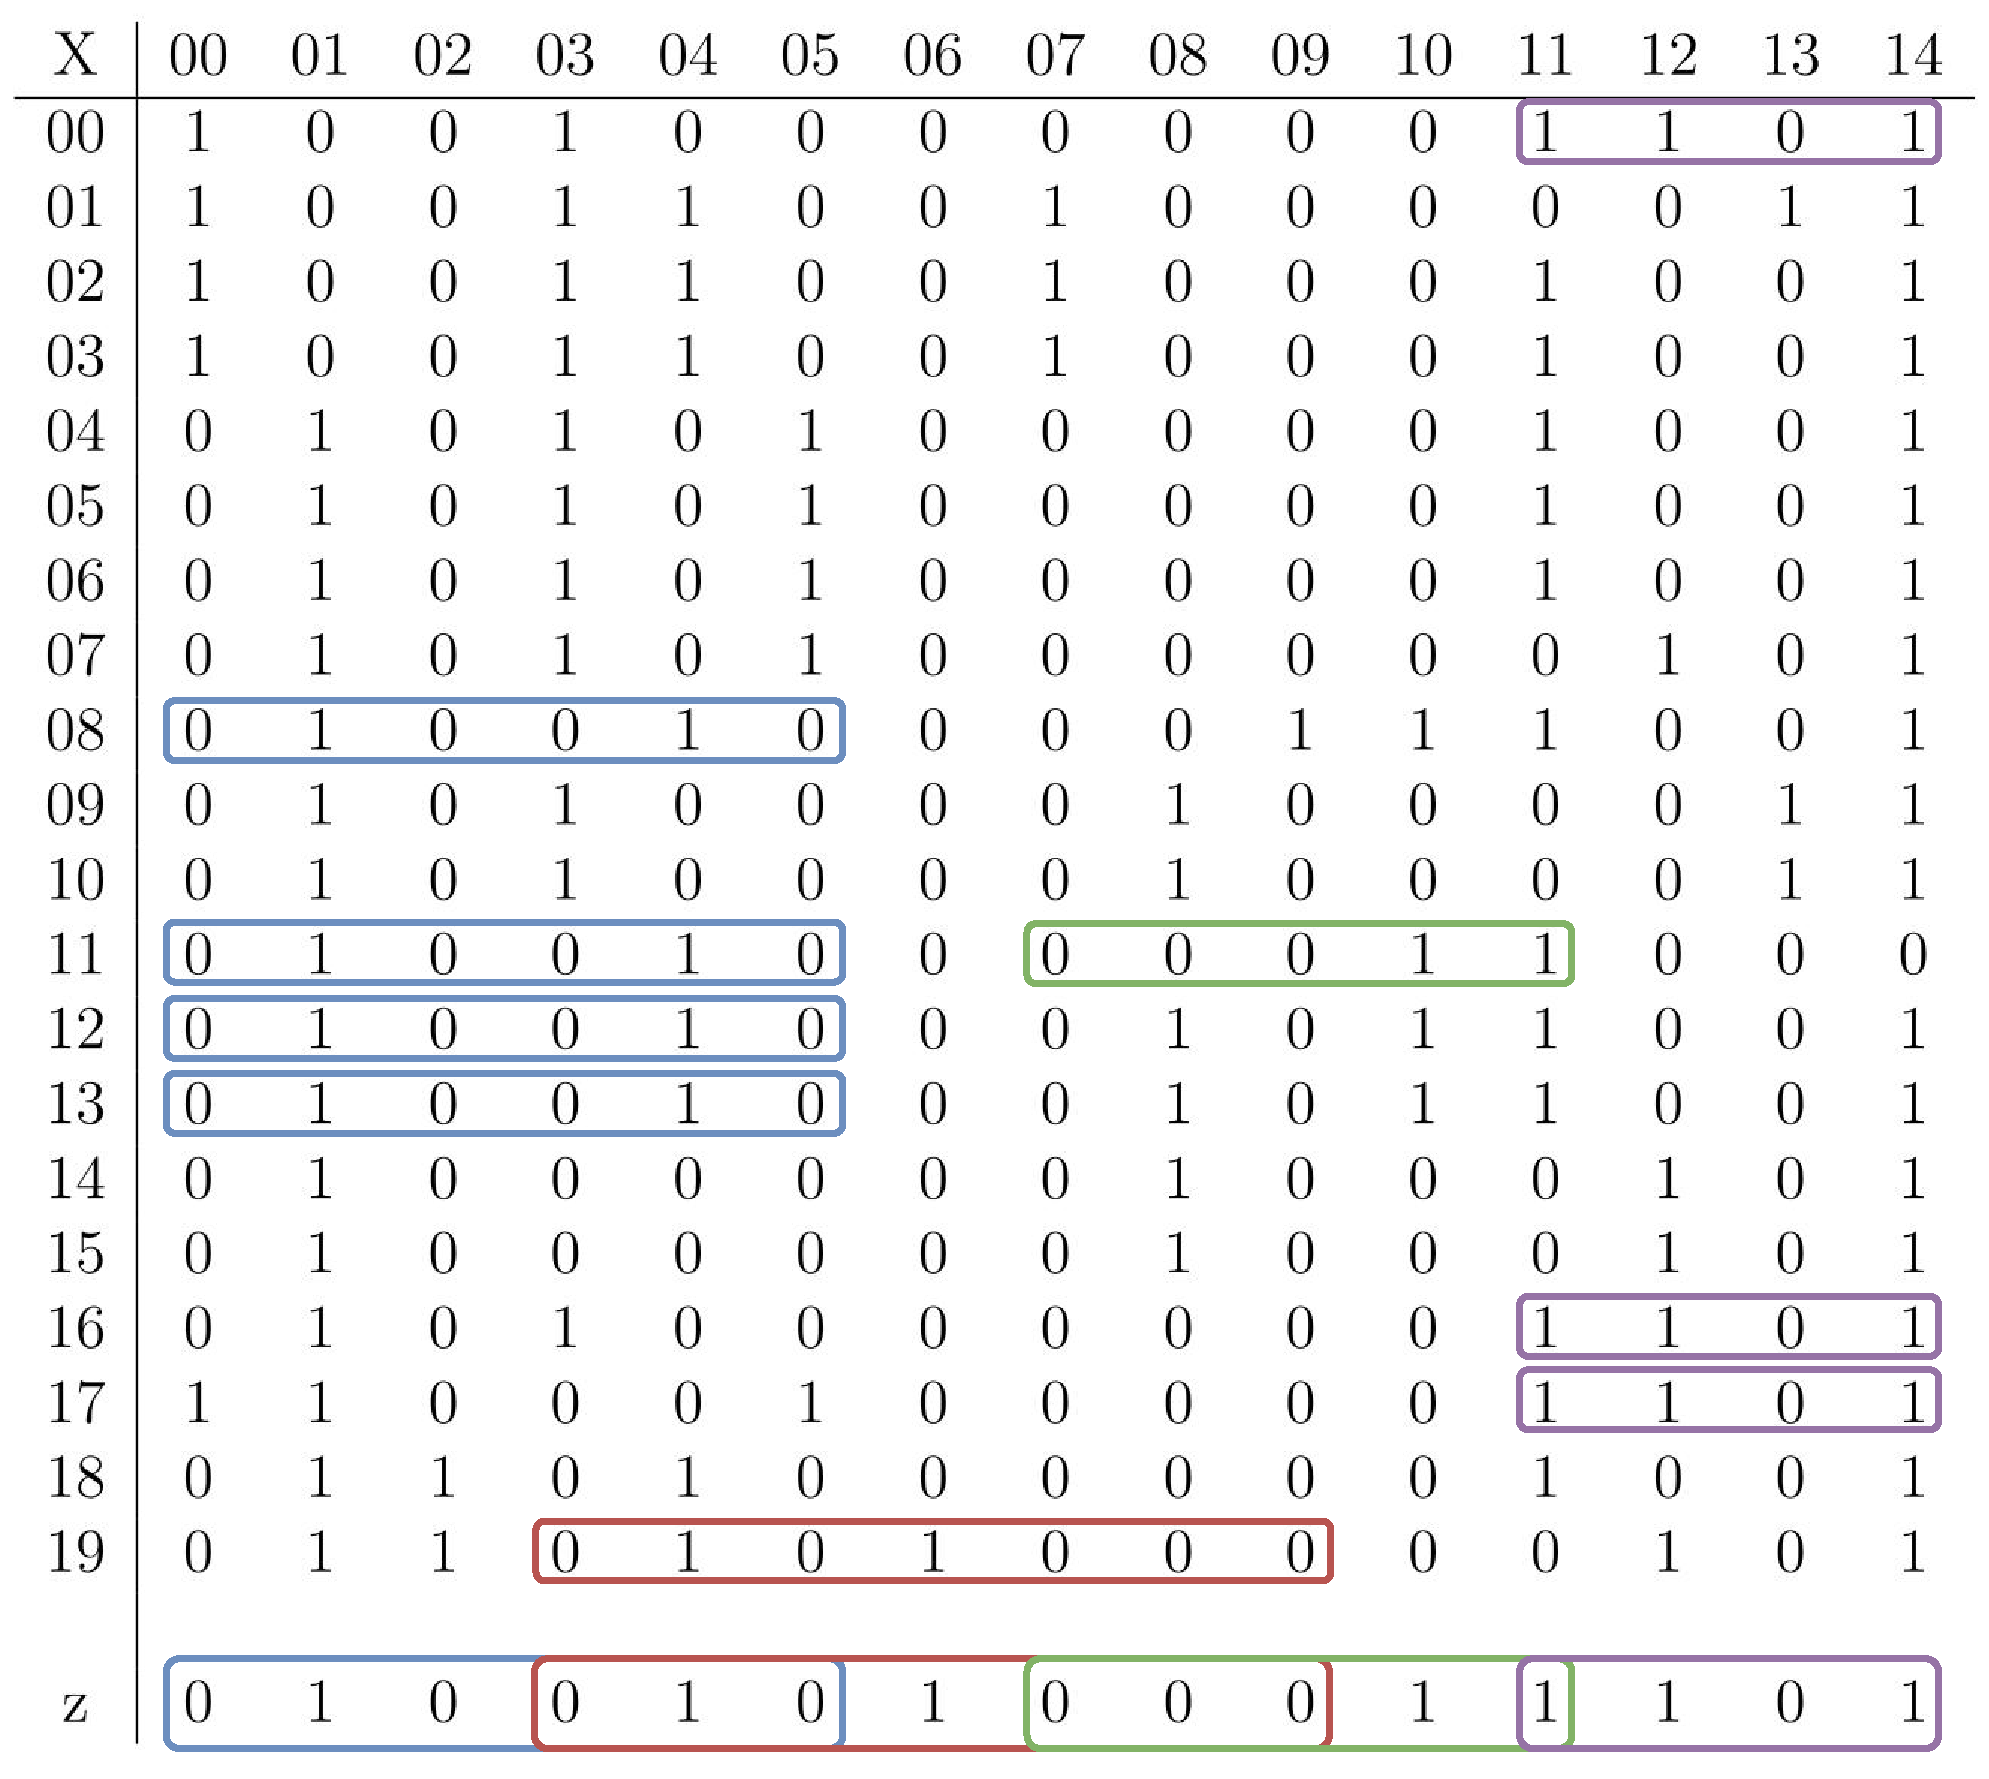
\includegraphics[scale = 0.365]{img/pbwtmatch.pdf}
  \end{figure}
  Si assuma di essere in colonna $k=6$, avendo, dopo i calcoli fatti in colonna
  $k=5$: 
  \begin{itemize}
    \item $f_6=6$
    \item $g_6=10$
    \item $e_6=0$
  \end{itemize}
  Avendo quindi che, a partire dalla colonne $0$ fino alla colonna $6-1=5$, si
  hanno le righe nel range $[6,10)$ di $a_{6}$ che matchano con $z[0,5]$. Tali
  righe sono, nel dettaglio, quelle indicizzate $\{8, 11, 12, 13\}$.\\
  Bisogna quindi aggiornare $f_7$ e $g_7$. Si assuma che $z[6]=1$ e che:
  \[y^6=00000000000100000000,\,\,\,c[6]=19\]
  Si calcolano quindi:
  \[f_7=w_6(6,1)=v_6[6]+c[6]=0+19=19\]
  \[g_7=w_6(10,1)=v_6[10]+c[6]=0+19=19\]
  Avendo quindi $f_7=g_7$ si procede, in primis, annotando i match terminanti in
  $k=5$.\\
  Seguendo l'algoritmo si ha quindi un primo aggiornamento di $e_{k+1}$, che
  viene inizializzato a, avendo in memoria $d_7$: 
  \[e_7=d_7[19]-1=7-1=6\]
  Questo viene fatto in quanto, come detto, l'aplotipo $z$ si trova o subito
  prima del blocco di aplotipi $[f_k,g_k)$.\\
  Essendo inoltre $z[e_7]=z[6]=1$ si procede aggiornando $g_7$ e tenendo fermo
  $f_7$, avendo $z[6]=1$. Si procede quindi inizializzando il
  nuovo $g_7$:
  \[g_7=f_7+1=20\]
  ricordando che $g_k$ può ``superare'' le dimensioni del pannello essendo
  escluso in $[f_k,g_k)$.\\
  A questo punto si segue la linea specificata da $f_7$ in $a_7$ a ritroso,
  partendo da $e_7-1$, fino a che si hanno match con $z$, aggiornando così il
  valore di $e_7$.\\
  In questo caso non si hanno altre operazioni, in quanto $g_7=M$ ma, qualora
  non lo fosse stato, si sarebbe incrementato $g_7$ fino a che il corrispondente
  $d_7[g_7]$ sarebbe stato minore o uguale di $e_7$, identificando tutte le
  nuove righe che hanno un match da con $z[e_7, 6]$.
  \dc{Forse sono necessarie immagini?}
\end{esempio}
L'\textit{algoritmo 5}, consultabile all'algoritmo \ref{algo:dur5} secondo i
calcoli di Durbin, ha complessità:
\begin{equation}
  \label{eq:pbwtsmem5}
  \mathcal{O}(N+c)
\end{equation}
tale risultato è stimato tale in quanto si ritiene che il
numero di accessi ai loop interni sia limitato dalla costante rappresentante il
numero di match, $c$. Nonostante ciò tale complessità temporale è ancora in
corso di studio in quanto si hanno in letteratura evidenze della sua non
correttezza. Un esempio è il paper di Naseri \cite{dpbwt}, dove si afferma che
l'intuizione per cui tale costante $c$ limiti superiormente gli accessi ai loop
innestati sia falsa. Si noti che nell'articolo non viene però precisata una
nuova misura per la complessità dell'algoritmo ma solo che la stima di Durbin è
empiricamente accettabile come \textit{caso medio}:
\begin{equation}
  \label{eq:pbwtsmem6}
  Avg.\,\,\,\mathcal{O}(N+c)
\end{equation}
In ogni caso, una soluzione na\"{i}ve, impiegherebbe tempo:
\begin{equation}
  \label{eq:pbwtsmem7}
  \mathcal{O}(N^2M)
\end{equation}
Si comprende, quindi, come tale algoritmo e tale struttura siano stati
rivoluzionari per lo studio di pannelli di aplotipi.
\begin{algorithm}
  \begin{algorithmic}[1]   
    \Function{Find\_Set\_Maximal\_Matches\_With\_Z}{$z$}
    \State $e\gets 0,\,\,f\gets 0,\,\,f\gets 0$
    \For {$k\gets 0$ \textbf{to} $N$}
    \State $e,f,g\gets \mbox{\textit{Update\_Matches}}(k, z, e, f, g)$
    \EndFor
    \EndFunction
    \State
    \Function{Update\_Matches}{$k, z, e, f, g$}
    \State $f'\gets \W(k, f, z[k])$
    \State $g'\gets \W(k, g, z[k])$
    \If{$f'<g'$}
    \Comment\textit{{se $k$ è $N-1$ report degli $\SMEM$ da $e_k$ a $N-1$}}
    \State $e'\gets e_k$
    \Else
    \Comment{\textit{report degli $\SMEM$ da $e_k$ a $k$}}
    \State $e'\gets d_{k+1}[f']-1$
    \If{$z[e']=0$ \textbf{and} $f'>0$}
    \State $f'\gets g'-1$
    \State \textbf{while} $z[e'-1]=y_{f'}^{k+1}[e'-1]$ \textbf{do} $e'\gets
    e'-1$
    \State \textbf{while} $d_{k+1}[f']\leq e'$ \textbf{do} $f'\gets f'-1$
    \Else
    \State $g'\gets f'+1$
    \State \textbf{while} $z[e'-1]=y_{f'}^{k+1}[e'-1]$ \textbf{do}  $e'\gets
    e'-1$ 
    \State \textbf{while} $g'<M$ \textbf{and} $d_{k+1}[g']\leq e'$ \textbf{do}
    $g'\gets g'+1$ 
    \EndIf
    \EndIf
    \State \textbf{return} $e',f',g'$
    \EndFunction
  \end{algorithmic}
  \caption{\footnotesize{Algoritmo 5 di Durbin per il calcolo degli $\SMEM$ con
  aplotipo esterno.}}
  \label{algo:dur5}
\end{algorithm}
\subsubsection{Limiti spaziali}
Bisogna affrontare la tematica della complessità in spazio di tale
algoritmo. Si ipotizzi di non ricalcolare, colonna per colonna, comportando
un'incremento dal punto di vista temporale in caso di dover studiare più query
$z$, tutti gli array  
necessari a costruire la $\PBWT$ e a permettere di computare la funzione
$\W(i,\sigma)$.\\
Ricapitolando, per poter eseguire l'algoritmo 5, si necessita di avere in
memoria, con \textit{random access}:
\begin{itemize}
  \item il \textbf{pannello} $X$, di dimensione $NM$
  \item l'insieme dei \textbf{prefix array} $a$, di dimensione $NM$
  \item l'insieme dei \textbf{divergence array} $d$, di dimensione $NM$
  \item i \textbf{vettori} $u_k$ e $v_k$, per ogni colonna $k$, complessivamente
  di dimensione $2NM$ 
  \item il \textbf{vettore} $c$, di dimensione $N$
\end{itemize}
Possiamo quindi dire che si ha una complessità in memoria pari a:
\begin{equation}
  \label{eq:pbwtsize}
  \mathcal{O}(NM)
\end{equation}
Nel dettaglio, Durbin stesso ha proposto una stima quantitativa di tale memoria
richiesta,
ovvero\footnote{\scriptsize{\url{https://github.com/richarddurbin/pbwt/blob/0de8d02df1b77146ded81e9e196991fdab520767/pbwtMatch.c\#L252}}}:
\begin{equation}
  \label{eq:pbwtsize2}
  13NM\mbox{ byte}
\end{equation}
Per poter capire meglio la problematica conseguente a tali richieste di spazio,
prendiamo, ad esempio, un pannello di 
dimensioni $N= 6.196.151$ e $M=4.908$. Ne segue che, secondo la stima
di 
Durbin, si necessitano 368GB di memoria. Una stima
sperimentale di tale richiesta di memoria può essere confermata con l'esecuzione
dell'implementazione ufficiale della
$\PBWT$\footnote{\url{https://github.com/richarddurbin/pbwt}}. Infatti,
monitorando  
con \texttt{time} il picco di memoria durante l'esecuzione, si ha che esso
corrisponde a 369GB, comprensivi anche di tutto ciò che è ``a
contorno'' all'algoritmo stesso. I dati quindi sembrano confermare le stime di
Durbin, confermando l'alto uso di memoria richiesto dall'\textit{algoritmo
  5}. Questa è 
stata la motivazione principale per cui si è sviluppata, in questa tesi
magistrale, una versione run-length encoded della $\PBWT$ che permettesse il
calcolo degli $\SMEM$ con un aplotipo esterno, in modo efficiente dal punto di
vista della memoria richiesta.
\subsection{Varianti della PBWT}
Negli anni immediatamente successivi all'articolo di Durbin, una miriade di
articoli e ricerche sono state svolte per migliorare la $\PBWT$, crearne
varianti o utilizzarla per portare a compimento vari studi. Non essendo tali
lavori direttamente correlati a questa tesi non 
verranno approfonditi ma, soprattutto nell'ottica dei prospetti futuri, è bene
citarne i principali.
\subsubsection{PBWT multiallelica}
La prima variante che si introduce è la \textbf{PBWT multiallelica} ($\MPBWT$),
proposta da Naseri et al. nel 2019 \cite{mpbwt}. Questo 
lavoro estende la $\PBWT$ di Durbin generalizzandola ad un alfabeto
arbitrario. \\
Dal punto di vista delle motivazioni biologiche, questa soluzione risulta
fondamentale, oltre che per lo studio di specie multialleliche (soprattutto nel
mondo vegetale), in quanto gli studi riportano come, nell'uomo, la presenza di
siti triallelici sia sotto stimata. \\
Da un punto di vista prettamente algoritmico si sono quindi estesi i concetti di
$c$, $u_k$ e $v_k$ visti nella $\PBWT$ per ottenere un vero e proprio
FM-index in grado di lavorare su alfabeto arbitrario $\Sigma$, con
conseguente forte aumento dello spazio richiesto in memoria. Da un punto di
vista della complessità temporale, invece, si ha che le le stime asintotiche
degli 
algoritmi devono tenere conto anche della grandezza dell'alfabeto stesso, avendo
però che, essendo esso tendenzialmente di dimensioni ridotte, questo fatto non
comporti particolari problematiche dal punto di vista dei tempi di
calcolo. Infatti, le complessità temporali della $\MPBWT$ sono incrementate
di un fattore $t$, con $t=\left|\Sigma\right|$, e se tale valore è assunto
costante ad inizio computazione, avendo che difficilmente si ha $t>>2$, la
complessità temporale non subisce variazioni considerevoli.
\subsubsection{PBWT con struttura LEAP}
Sempre nel 2019, Naseri et al.\cite{leap} proposero anche una variante della
$\PBWT$ 
che permettesse il calcolo non solo degli $\SMEM$, come per l'algoritmo 5
di Durbin, ma anche qualsiasi match di lunghezza maggiore uguale ad una
lunghezza arbitraria $L$. Tale algoritmo fu nominato
\textit{PBWT-query}. Inoltre, nello 
stesso articolo, proposero 
una struttura dati aggiuntiva, detta \textit{LEAP} (Linked
Equal/Alternating Position), che, al costo della 
memorizzazione di otto array aggiuntivi che permettessero di effettuare dei
salti nella matrice $\PBWT$ (salvando gli indici del precedente/prossimo
valore nella colonna uguale/diverso) e di memorizzare gli indici dei valori
nel divergence array relativi a tali indici, ottimizzava i tempi
dell'algoritmo per la PBWT-query, ottenendo l'algoritmo detto
\textit{L-PBWT-query}.
\dc{Serve dire di più sulla struttura LEAP?}
Da un punto di vista computazionale, si noti che la complessità in tempo
dell'algoritmo 
per la PBWT query, con match di lunghezza minima $L$ è:
\begin{equation}
  \label{eq:leap1}
  \mathcal{O}(N+c(R-L+1))
\end{equation}
Avendo:
\begin{itemize}
  \item $R$ lunghezza media dei match
  \item $c$ numero totale dei match
\end{itemize}
In merito ai tempi dell'algoritmo L-PBWT-query si ha che, al
costo di $8NM$ interi aggiuntivi in memoria, con $N$ e $M$ dimensioni del
pannello è proporzionale a: 
\begin{equation}
  \label{eq:leap2}
  \mathcal{O}(N+c)
\end{equation}
\subsubsection{PBWT dinamica}
Sanaullah et al., nel 2021, proposero la \textbf{Dynamic PBWT} ($\DPBWT$)
\cite{dpbwt} col fine di superare le limitazioni imposte dalle strutture
statiche usate nella $\PBWT$ di Durbin. Si è quindi pensato di sostituire
l'uso degli array, statici, con l'uso di linked list, ovvero strutture dati
dinamiche.\\ 
Grazie alle linked list, si è reso possibile l'aggiornamento
efficiente della matrice $\PBWT$ all'aggiunta di un nuovo aplotipo nel
pannello o alla rimozione di uno già presente nel pannello.\\
Da un punto di vista computazionale, è interessante notare come le
implementazioni degli algoritmi di Durbin presentino la medesima complessità
asintotica. Infatti, ad esempio, la creazione della $\DPBWT$ richiede
tempo:
\begin{equation}
  \label{eq:dpbwt}
  \mathcal{O}(NM)
\end{equation}
Invece, l'aggiunta e la rimozione di un aplotipo sono entrambe in tempo:
\begin{equation}
  \label{eq:dpbwt1}
  Avg.\,\,\,\mathcal{O}(N)
\end{equation}
\subsubsection{PBWT con wildcard}
La tematica dei dati mancanti è una tematica aperta in
bioinformatica. I sequenziatori infatti presentano un range d'errore
dal 1\% al 15\%, si ha a volte un basso coverage (ovvero il numero di
read che contengono la base sequenziata per un certo locus del genoma) e la fase
di assemblaggio del genoma può comportare errori. Questo, in fase di produzione
dei pannelli, implica che, in determinati casi, non si sappia quale sia l'allele
corretto per un individuo riferendosi ad un sito. \\
Nel 2020, Williams e Mumey \cite{williams} proposero quindi l'uso della
$\PBWT$ \textbf{con 
  wildcard} al fine di disegnare un algoritmo in grado di calcolare i match
interni ad un pannello biallelico con dati mancanti, rappresentati come
wildcard mediante il simbolo ``*'' (avendo quindi
$\Sigma=\{0,1,*\}$).\\ 
In termini computazionali gli autori sono riusciti a formulare un algoritmo in
grado tutti i match interni massimali al pannello in
tempo, con $T$ numero di match: 
\begin{equation}
  \label{eq:pbwtwild}
  \mathcal{O}(NMT)
\end{equation}
\dc{Serve dire altro? Ho evitato di citare il termine blocco per non dover
  aggiungere la definizione}
\subsubsection{IMPUTE5}
Per citare un uso della $\PBWT$, si può introdurre il concetto di
\textit{genotype 
  imputation}, ovvero il processo con il quale si predicono genotipi non ancora
osservati in un campione di individui, usando un pannello di aplotipi. Questo
tipo di studio si basa sui dati prodotti dai \textbf{GWAS} (Genome-wide
    association studies), studi il cui scopo è quello di di esaminare multipli
genomi alla ricerca di associazioni tra varianti genetiche e malattie (o
outcome specifici delle stesse), identificando varianti genomiche che sono
statisticamente associate al rischio per una malattia.\\ 
A tal fine, nel 2020, Rubinacci et al. proposero \textbf{IMPUTE5}
\cite{impute5}, un metodo basato sulla $\PBWT$ per la genotype
  imputation, in grado di studiare pannelli di grandi dimensioni.
\dc{Aggiungere qualcosa?}
\subsection{Una prima proposta run-length encoded}
\label{subsectravis}
A fine 2021, Gagie et al. \cite{tricks} hanno iniziato a teorizzare una variante
run-length encoded della $\PBWT$, cercando di basarsi sui risultati
già ottenuti sulla $\BWT$ con la $\RLBWT$.\\
Pensando alla costruzione della $\PBWT$, con $M$ individui e $N$ siti, si
ha che ogni colonna della 
matrice $\PBWT$ è ottenuta tramite la permutazione data dal prefix
  array. Denotiamo tale permutazione, alla colonna $k$, con $\pi_k$, $\forall\,
1\leq k<N$. 
Ipotizziamo ora di voler studiare la riga $i$-esima del pannello originale. Si
ha che, al variare della colonna $k$ sulla matrice $\PBWT$, la posizione
della riga $i$ è ricostruibile applicando le varie permutazioni:
\begin{equation}
  \label{eq:pbwttrick}
  i, \pi_1(i), \pi_2(\pi_1(i)),\ldots,
  \pi_{N-1}(\cdots(\pi_2(\pi_1(i)))\cdots)
\end{equation}
Il punto fondamentale si ritrova nel fatto che l'autore asserisce:
\begin{center}
  \textit{Notice $\pi_k$ can be stored in space proportional to the number of
    runs in the $k$th column of the $\PBWT\,\ldots$} 
\end{center}
Nell'articolo si propone una struttura dati formata da $N$ ``tabelle''
dove, la $j$-esima riga della $k$ tabella contiene: 
\begin{itemize}
  \item l'indice $p$ di inizio della $j$-esima run nella colonna $k$ della
   matrice $\PBWT$
  \item il valore $\pi_k(p)$, avendo che:
  \begin{equation}
    \label{eq:pbwttrick1}
    \pi_k(p)=
    \begin{cases}
      p-v_k[p]&\mbox{if } y_p^k[k]=0\\
      c[k]+v_k[p]-1&\mbox{if } y_p^k[k]=1\\
    \end{cases}
  \end{equation}
  \item l'indice della run contenente il simbolo $\pi_k(p)$ nella colonna $k+1$
  della matrice $\PBWT$
  \item un booleano per capire se la prima run è composta da simboli $\sigma=0$
  o $\sigma =1$. Si noti che tale valore non è esplicitato nel'articolo ma
  risulta necessario
\end{itemize}
Il paper presenta anche il metodo per l'estrazione della $i$-esima
riga. Inizialmente, si cerca della prima ``tabella'' la riga relativa alla run,
con indice di testa $p$, contenente l'indice $i$. Si noti che la prima
``tabella'', relativa alla colonna $k=0$ non presenta permutazioni e quindi  
l'indice $i$ del pannello è anche l'indice $i$ della matrice $\PBWT$.
Si può calcolare, quindi, la permutazione per l'indice $i$ (alla prima
operazione si avrà $k=1$):
\begin{equation}
  \label{eq:pbwttrick2}
  \pi_k(i)=\pi_k(p)+i-p
\end{equation}
Si identifica, poi, la riga relativa alla run contenente il simbolo $\pi_k(p)$
nella ``tabella'' successiva e si scansionano le righe di tale tabella a
partire da quella appena identificata fino a trovare la run che contiene
$\pi_k(i)$ (alla prima
operazione si avrà $k=1$). Infine, si estrae il simbolo relativo a tale run.
Ripetendo la procedura, per ogni colonna $k$, dal computo della permutazione, si
può calcolare la riga $i$-esima del pannello.\\
Inoltre,
vengono proposti ulteriori ottimizzazioni, basate sul metodo detto
\textit{fractional cascading}. Con tale rappresentazione, si riesce a ridurre il
numero di run che devono essere scansionate nel passaggio 3, al costo di una
maggior richiesta di spazio. Infatti, aumentando il numero totale di
righe in tutte le tabelle di un fattore al più $\left(1+\frac{1}{d}\right)$, è
possibile garantire che si avranno al più $d$ iterazioni, in ogni tabella, per
ottenere l'estrazione del simbolo desiderato.
Per ulteriori dettagli si rimanda al paper di riferimento \cite{tricks}.
\begin{esempio}
   Supponendo di voler ricostruire la riga $i=9$, si assuma la seguente matrice
   $\PBWT$, avendo che in rosso sono segnati i simboli appartenenti alla riga 9: 
   \begin{table}[H]
     \centering
     \footnotesize
     \begin{tabular}{c|ccccccccccccccc}
       X & 01 & 02 & 03 & 04 & 05 & 06 & 07 & 08 & 09 & 10 & 11 & 12 \\
       \hline
       00 & 1 & 1 & 0 & 0 & 0 & 1 & 0 & 0 & 1 & 1 & 1 & 1 \\
       01 & 1 & 1 & 0 & 0 & 0 & 1 & 0 & 0 & 1 & 1 & {\color{nordred}\textbf{\underline{1}}}
                                                                & 1 \\
       02 & 1 & 1 & 1 & 0 & 0 & 0 & 1 & 1 & 1 & 0 & 1 & 1 \\
       03 & 1 & 1 & 0 & {\color{nordred}\textbf{\underline{0}}} & {\color{nordred}\textbf{\underline{0}}}
                                  & {\color{nordred}\textbf{\underline{1}}} & 0 & 0 & 1 & 1
                                                           & 0 & 1 \\
       04 & 1 & 0 & 1 & 0 & 0 & 1 & 0 & 0 & 1 & 1 & 0 & 1 \\
       05 & 1 & 0 & 1 & 0 & 0 & 0 & 0 & 0 & 1 & {\color{nordred}\textbf{\underline{0}}} & 0
                                                                & 1 \\
       06 & 1 & 0 & 1 & 0 & 0 & 0 & 0 & 0 & 1 & 0 & 0 & 0 \\
       07 & 1 & 1 & 1 & 0 & 0 & 0 & 0 & 0 & 0 & 1 & 0 & 1 \\
       08 & 0 & 1 & {\color{nordred}\textbf{\underline{0}}} & 0 & 0 & 1 & 0 & 0 & 0 & 1 & 0
                                                                & 1 \\
       09 & {\color{nordred}\textbf{\underline{1}}} & 0 & 0 & 0 & 0 & 1 & 0 & 0 & 0 & 0 & 0
                                                                & 1 \\
       10 & 1 & 1 & 0 & 0 & 0 & 0 & 0 & 0 & 1 & 1 & 0 & 1 \\
       11 & 0 & 1 & 0 & 1 & 1 & 0 & 0 & 0 & 1 & 0 & 0 & 1 \\
       12 & 0 & 1 & 0 & 0 & 1 & 0 & 0 & 0 & 0 & 0 & 0 & 1 \\
       13 & 0 & 0 & 0 & 0 & 1 & 0 & 0 & 0 & 0 & 0 & 0 & 1 \\
       14 & 0 & 0 & 0 & 0 & 0 & 0 & 0 & 0 & {\color{nordred}\textbf{\underline{0}}} & 0 & 0
                                                                & 1 \\
       15 & 0 & 0 & 0 & 0 & 0 & 0 & 0 & {\color{nordred}\textbf{\underline{0}}} & 0 & 0 & 0
                                                                & 1 \\
       16 & 1 & 0 & 0 & 0 & 0 & 0 & {\color{nordred}\textbf{\underline{0}}} & 0 & 1 & 0 & 0
                                                                & 1 \\
       17 & 0 & {\color{nordred}\textbf{\underline{0}}} & 0 & 0 & 0 & 0 & 0 & 1 & 1 & 0 & 0
                                                                & 1 \\
       18 & 0 & 0 & 0 & 0 & 0 & 0 & 0 & 1 & 1 & 0 & 0
                                                                & {\color{nordred}\textbf{\underline{1}}} \\ 
       19 & 0 & 0 & 0 & 0 & 0 & 0 & 0 & 1 & 1 & 0 & 0 & 1 \\
     \end{tabular}
   \end{table}
   \noindent
   Si costruiscono quindi le seguenti tabelle \cite{tricks}:
   \begin{figure}[H]
     \centering
     %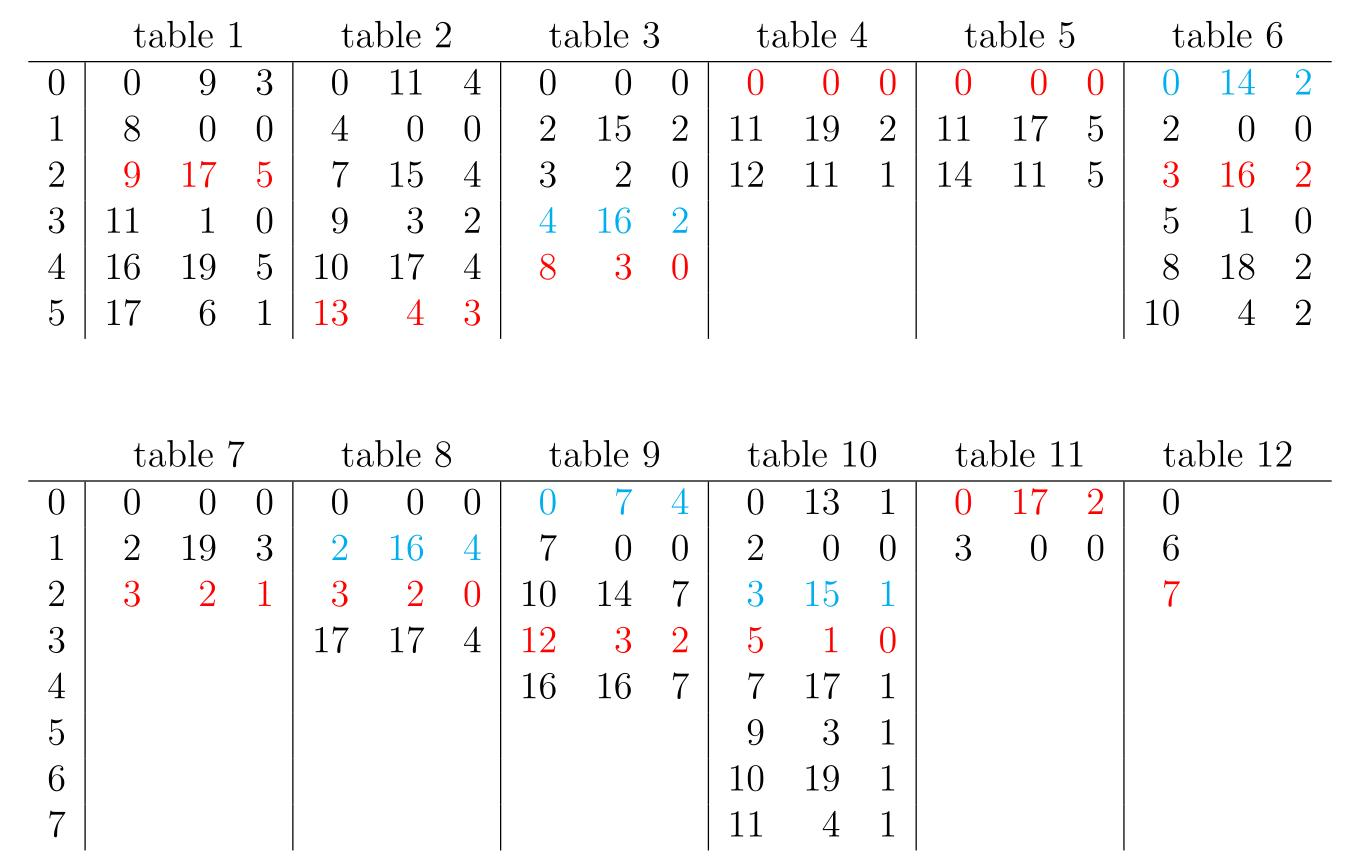
\includegraphics[scale=0.3]{img/trick.jpg}
     %\resizebox{0.75\textwidth}{!}
     {\begin{tabular}{r|rrr|rrr|rrr|rrr|rrr|rrr}
        \multicolumn{1}{c}{} &
                               \multicolumn{3}{c}{table 1} &
                                                             \multicolumn{3}{c}{table 2} &
                                                                                           \multicolumn{3}{c}{table 3} &
                                                                                                                         \multicolumn{3}{c}{table 4} &
                                                                                                                                                       \multicolumn{3}{c}{table 5} &
                                                                                                                                                                                     \multicolumn{3}{c}{table 6} \\
        \hline
        0 &  0 &  9 &  3 &  0 & 11 &  4 &  0 &  0 &  0 &  \textcolor{nordred}{0} &  \textcolor{nordred}{0} &  \textcolor{nordred}{0}
                                        &  \textcolor{nordred}{0} &  \textcolor{nordred}{0} &  \textcolor{nordred}{0}
                                                       &  \textcolor{nordcyan}{0} & \textcolor{nordcyan}{14} &  \textcolor{nordcyan}{2} \\
        1 &  8 &  0 &  0 &  4 &  0 &  0 &  2 & 15 &  2 & 11 & 19 &  2 & 11 & 17 &  5 &  2 &  0 &  0 \\
        2 &  \textcolor{nordred}{9} & \textcolor{nordred}{17} &  \textcolor{nordred}{5}
                                                                                                                       &  7 & 15 &  4 &  3 &  2 &  0 & 12 & 11 &  1 & 14 & 11 &  5 &  \textcolor{nordred}{3} & \textcolor{nordred}{16} &  \textcolor{nordred}{2} \\
        3 & 11 &  1 &  0 &  9 &  3 &  2 &  \textcolor{nordcyan}{4} & \textcolor{nordcyan}{16} &  \textcolor{nordcyan}{2}
                         &    &    &    &    &    &    &  5 &  1 &  0 \\
        4 & 16 & 19 &  5 & 10 & 17 &  4 &  \textcolor{nordred}{8} &  \textcolor{nordred}{3} &  \textcolor{nordred}{0}
                         &    &    &    &    &    &    &  8 & 18 &  2 \\
        5 & 17 &  6 &  1 & \textcolor{nordred}{13} &  \textcolor{nordred}{4} &  \textcolor{nordred}{3}
          &    &    &    &    &    &    &    &    &    & 10 &  4 &  2 \\
        \multicolumn{7}{c}{} \\[3ex]
        \multicolumn{1}{c}{} &
                               \multicolumn{3}{c}{table 7} &
                                                             \multicolumn{3}{c}{table 8} &
                                                                                           \multicolumn{3}{c}{table 9} &
                                                                                                                         \multicolumn{3}{c}{table 10} &
                                                                                                                                                        \multicolumn{3}{c}{table 11} &
                                                                                                                                                                                       \multicolumn{3}{c}{table 12} \\
        \hline
        0 &  0 &  0 &  0 &  0 &  0 &  0 &  \textcolor{nordcyan}{0} &  \textcolor{nordcyan}{7} &  \textcolor{nordcyan}{4}
                         &  0 & 13 &  1 &  \textcolor{nordred}{0} & \textcolor{nordred}{17} &  \textcolor{nordred}{2}
                                                       &  0 & \\
        1 &  2 & 19 &  3 &  \textcolor{nordcyan}{2} & \textcolor{nordcyan}{16} &  \textcolor{nordcyan}{4}
          &  7 &  0 &  0 &  2 &  0 &  0 &  3 &  0 &  0 &  6 & \\
        2 &  \textcolor{nordred}{3} &  \textcolor{nordred}{2} &  \textcolor{nordred}{1}
                                                                                                                       &  \textcolor{nordred}{3} &  \textcolor{nordred}{2} &  \textcolor{nordred}{0}
          & 10 & 14 &  7 &  \textcolor{nordcyan}{3} & \textcolor{nordcyan}{15} &  \textcolor{nordcyan}{1}
                                        &    &    &    &  \textcolor{nordred}{7} & \\
        3 &    &    &    & 17 & 17 &  4 & \textcolor{nordred}{12} &  \textcolor{nordred}{3} &  \textcolor{nordred}{2}
                         &  \textcolor{nordred}{5} &  \textcolor{nordred}{1} &  \textcolor{nordred}{0} &    &    &    &    & \\
        4 &    &    &    &    &    &    & 16 & 16 &  7 &  7 & 17 &  1 &    &    &    &    & \\
        5 &    &    &    &    &    &    &    &    &    &  9 &  3 &  1 &    &    &    &    & \\
        6 &    &    &    &    &    &    &    &    &    & 10 & 19 &  1 &    &    &    &    & \\
        7 &    &    &    &    &    &    &    &    &    & 11 &  4 &  1 &    &    &    &    &
      \end{tabular}
    }

  \end{figure}
  Nelle tabelle, in rosso, si hanno le varie $\pi_k(i)$ calcolate nel processo,
  ottenute, 
  se necessario, iterando a partire dalle $\pi_k(p)$, segnalate in azzurro. \\
  Si hanno infatti i seguenti calcoli, ovvero i vari $\pi_j(i)=\pi_j(p)+i-p$ 
  relativi alle permutazioni in colonna $k$, per l'estrazione della riga $9$:
  \begin{multicols}{2}
    \begin{itemize}
      \item $\pi_1(9)=17+9-9=17$
      \item $\pi_2(17)=4+17-13=8$
      \item $\pi_3(8)=4+8-8=3$
      \item $\pi_4(3)=0+3-0=3$
      \item $\pi_5(3)=0+3-0=3$
      \item $\pi_6(3)=16+3-3=16$
      \item $\pi_7(16)=2+16-3=15$
      \item $\pi_8(15)=2+15-3=14$
      \item $\pi_9(14)=3+14-12=5$
      \item $\pi_{10}(5)=1+5-5=1$
      \item $\pi_{11}(1)=17+1-0=18$
      % \item $\pi_{12}(3)=16+3-3=16$        
    \end{itemize}
  \end{multicols}
  Sfruttando quindi il valore booleano (non rappresentato nelle tabelle ma
  necessario in memoria) che ci dice con che simbolo inizia una colonna
  della matrice $\PBWT$ e
  sapendo che, 
  essendo un pannello binario, si alternano run con simboli $\sigma=0$ e
  $\sigma=1$, si può ricostruire la riga 9 del pannello originale:
  \[x_9=100001000011\]
\end{esempio}
Si segnala che, nel paper, non vengono specificati metodi per
effettuare query a 
tale struttura dati, indicando solo che dovrebbe essere possibile interrogare
tale struttura a tabelle.
% LocalWords:  pseudocodice aplotipi mismatch
